In questo capitolo sono analizzate le componenti del processo di correzione, con lo scopo di capire quali sono i limiti del sistema e quali siano le parti che più causano un collo di bottiglia alle performance di correzione.\\
Nella \autoref{sec:ana_intro} sono date le motivazioni che hanno portato allo svolgimento di questa analisi, della quale è illustrata rapidamente la metodologia. Nella \autoref{sec:ana_dst} è descritto il processo di modifica del dataset esistente per renderlo consono all'esecuzione dell'analisi. Nelle sezioni \ref{sec:ana_bert} e \ref{sec:ana_cor} sono riportate le metriche utilizzate per l'analisi e i risultati ottenuti.

\section{Introduzione}
\label{sec:ana_intro}
Nel \autoref{sec:test} sono esposti i risultati dei test sul sistema di correzione. I test svolti valutano le performance complessive del sistema, ma non danno alcuna indicazione rispetto alle fasi che lo compongono. Identificare quali sono le fasi che più influenzano negativamente o positivamente le performance di correzione può essere utile per capire quali sono le componenti da migliorare con più priorità per lo sviluppo del sistema.\\
L'analisi presentata in questo capitolo riguarda nello specifico la correzione dei word error (\autoref{sec:met_introduzione}), e tratta quindi del modulo di correzione token (\autoref{sec:met_tok_correct}). Come visto in precedenza, il modulo di correzione token opera in due fasi: error detection e error correction. L'analisi, che verte sulla fase di error correction, valuterà:
\begin{itemize}
\item La capacità del modello BERT di produrre la soluzione per la correzione fra i vari candidati. La presenza della soluzione fra i candidati è condizione necessaria per poter applicare la giusta correzione: è quindi importante capire qual è il limite superiore che la generazione dei candidati pone al processo di correzione.

\item La capacità del sistema di correzione di scegliere il candidato corretto, se presente, fra quelli proposti dal modello BERT. Verrà valutata anche la capacità del sistema di evitare di apportare correzioni nel caso BERT non produca la soluzione fra i candidati.
\end{itemize}
La valutazione di questi due step del processo di correzione permetterà di stabilire quali sono i margini di miglioramento nella fase di error correction, considerando il limite superiore imposto dalla generazione dei candidati del modello BERT. Questo, confrontato con i risultati dei testi illustrati nel \autoref{sec:test}, permetterà di valutare anche il margine di errore della fase di error detection.


\section{Creazione di un dataset specifico}
\label{sec:ana_dst}
Come spiegato nell'introduzione, l'analisi presentata in questo capitolo verte unicamente sulla parte di error correction. \E\ quindi chiaro come la metodologia dell'analisi deve prevedere un modo per escludere l'error detection dal processo di correzione. Ciò implica che è necessario disporre di frasi in cui gli errori sono in posizione nota, in modo da non dover fare error detection.

\paragraph{Metodologia} L'idea è quella di perturbare ulteriormente le frasi presenti in \dstb, introducendo un solo word error per frase. Il token perturbato non viene però reinserito nella frase, ma viene mascherato, permettendo così di conoscere la posizione dell'errore da correggere e di avere una frase già pronta per la generazione dei candidati.\\
Ad esempio, data la frase già perturbata:
\begin{center}
\textit{"Sarà n e c e s s a r i o uno sforzo straordinario per mobilitare le risorse."}
\end{center}
si introduce un ulteriore word error, e si maschera la posizione dell'errore, ottenendo la seguente tripletta:
\begin{enumerate}
\item Frase: \textit{"Sarà n e c e s s a r i o uno sforzo [MASK] per mobilitare le risorse."}
\item Token originale: \textit{"straordinario"}
\item Token perturbato: \textit{"strnordinnrio"}
\end{enumerate}
Quanto appena spiegato informalmente è un processo divisibile nelle seguenti fasi:
\begin{enumerate}
\item Estrazione
\item Perturbazione
\end{enumerate}

\paragraph{Estrazione}
Lo scopo di questa fase è quello di ottenere una lista di frasi perturbate con diverse superpipeline. Nel contesto di questo capitolo si intende una frase come una stringa senza l'aggiunta di ulteriori metadati. Per ogni sample $s \in \dstb$ è possibile estrarre due tipi di frase:
\begin{itemize}
\item La frase originale non perturbata, presente nel campo \textit{text}.
\item Una frase perturbata scelta dal campo \textit{perturbed}. Ogni frase perturbata è identificata dalla superpipeline usata per la sua perturbazione.
\end{itemize}
Si ottiene l'insieme delle frasi estratte $D_{extr}$ estraendo casualmente frasi da \dstb\ in modo da rispettare la distribuzione in \autoref{tab:ana_distr}:
\begin{table}[H]
\centering
\begin{tabular}{cccc}
\textbf{Tipo frase} & \textbf{Num. frasi} \\
\hline
text & 3500 \\
T1 & 3500 \\
T2 & 3500 \\
T3 & 3500 \\
S1 & 3500 \\
S2 & 3500 \\
S3 & 3500 \\
M1 & 3500 \\
M2 & 3500 \\
M3 & 3500 \\ 
\hline
\textbf{Totale} & \textbf{35000}
\end{tabular}
\caption{Distribuzione delle frasi estratte. Per "tipo" si intende \textit{text} se la frase non è perturbata; se invece la frase è perturbata il tipo corrisponde alla superpipeline utilizzata}
\label{tab:ana_distr}
\end{table}
Ogni frase è inoltre associata al suo tipo: in questo modo durante l'analisi sarà possibile valutare i risultati anche i base all'intensità della perturbazione.

\paragraph{Perturbazione}
Per ogni frase $f \in D_{extr}$ il primo passaggio nella fase di perturbazione consiste nel tokenizzare la frase. Si ottiene quindi una lista di token $T = [t_1,...,t_n]$. Questo passaggio si rende necessario in quanto si vuole introdurre un errore all'interno di un singolo token.\\
Fra lista di token ottenuta dalla tokenizzazione si individua un subset $P \subseteq T$ di token detti "perturbabili". Un token $t$ è considerato perturbabile se soddisfa le seguenti condizioni:
\begin{itemize}
\item Dato lo stesso vocabolario $V$ usato per l'error detection (\autoref{sec:met_tok_errdet}), $t \in V$.

\item $t$ è lungo almeno due caratteri.
\end{itemize}
Queste condizioni servono ad evitare di ri-perturbare un token che è già stato perturbato in precedenza o che deriva dallo split di un altro token. Si pensi ad esempio a una situazione in cui \textit{"papa"} viene perturbato come \textit{"p a p a"}: pur essendo \textit{"a"} presente nel vocabolario, non sarebbe corretto considerare \textit{"a"} come un token perturbabile.\\
Si sceglie quindi in modo casuale un solo token $t_p$ da perturbare dall'insieme $P$. Per perturbare $t_p$ si usa la funzione $f_{alternative}$ del modulo di characters replacement (\autoref{dst:modpert}). Quindi, si ha che:
\begin{equation}
t\prime_p = f_{alternative}(t_p)
\end{equation}
Successivamente si sostituisce $t_p$ nell'insieme $T$ con il token \textit{"[MASK]"}, ottenendo la lista di token $T\prime = [t_1,...,[MASK],...,t_n]$. Infine, si detokenizza $T\prime$ per ottenere la frase mascherata $f\prime$. \\
Alla fine di questa fase, per ogni frase $f \in D_{extr}$ è prodotta una tupla strutturata come in \autoref{tab:ana_tuplapert}:

\begin{table}[H]
\centering
\begin{tabular}{cc}
\textbf{Campo} & \textbf{Contenuto}\\ \hline
\textit{sent} & Frase originale mascherata ($f\prime$)\\
\textit{maskedTok} & Token che è stato mascherato ($t\prime_p$)\\
\textit{correctTok} & Token originale non perturbato ($t_p$)\\
\textit{pertSup} & Tipo di $f$ (\autoref{tab:ana_distr}) \\
\end{tabular}
\caption{Tupla prodotta per ogni frase $f$ dalla fase di perturbazione}
\label{tab:ana_tuplapert}
\end{table}
\noindent
L'insieme delle tuple risultanti ottenuto da questa fase è detto $D_{an}$.

\paragraph{Esempio} Si prenda ad esempio la frase fornita come esempio all'inizio di questa sezione, perturbata con la superpipeline S1:
\begin{center}
\textit{"Sarà n e c e s s a r i o uno sforzo straordinario per mobilitare le risorse."}
\end{center}
La fase di perturbazione ha inizio tokenizzando la frase:
\begin{center}
\textit{\underline{'Sarà'}, 'n', 'e', 'c', 'e', 's', 's', 'a', 'r', 'i', 'o', \underline{'uno'}, \underline{'sforzo'}, \underline{'straordinario'}, \underline{'per'}, \underline{'mobilitare'}, \underline{'le'}, \underline{'risorse'}, '.'}
\end{center}
Si può notare come siano stati sottolineati tutti i token perturbabili. Viene scelto casualmente il token \textit{'straordinario'}. Si produce quindi una versione perturbata del token scelto:
\begin{equation}
f_{alternative}(\textit{'straordinario'}) =  \textit{'strnordinnrio'}
\end{equation}
Si procede sostituendo il token perturbato con \textit{[MASK]} all'interno della lista dei token:
\begin{center}
\textit{'Sarà', 'n', 'e', 'c', 'e', 's', 's', 'a', 'r', 'i', 'o', 'uno', 'sforzo', '[MASK]', 'per', 'mobilitare', 'le', 'risorse', '.'}
\end{center}
Si detokenizza in seguito la lista di token:
\begin{center}
\textit{"Sarà n e c e s s a r i o uno sforzo [MASK] per mobilitare le risorse."}
\end{center}
Si produce quindi la tupla in \autoref{tab:ana_tuplaex}:
\begin{table}[H]
\centering
\begin{tabular}{cp{12cm}}
\textbf{Campo} & \textbf{Contenuto}\\ \hline
\textit{sent} & \textit{"Sarà n e c e s s a r i o uno sforzo [MASK] per mobilitare le risorse."}\\
\textit{maskedTok} & \textit{"strnordinnrio"}\\
\textit{correctTok} & \textit{"straordinario"}\\
\textit{pertSup} & S1 \\
\end{tabular}
\caption{Tupla prodotta per ogni frase $f$ dalla fase di perturbazione}
\label{tab:ana_tuplaex}
\end{table}


\section{Analisi generazione dei candidati}
\label{sec:ana_bert}
La generazione dei candidati è la prima parte dello stadio di candidates generation and picking della fase di error correction del modulo di correzione token (\autoref{sec:met_tok_correct}). La generazione dei candidati sfrutta un modello BERT allenato sul masked language modelling (\autoref{sec:met_BERT_MLM}), per produrre i possibili candidati al rimpiazzo del token [MASK] in una frase data in input. Si ricorda inoltre che ogni candidato prodotto da BERT è associato alla propria probabilità di essere il rimpiazzo corretto.

\paragraph{Metriche} L'analisi della generazione dei candidati mira quindi a quantificare la capacità del modello BERT di produrre la soluzione fra i candidati proposti. Si intende inoltre misurare quanto accurata sia la probabilità che il modello associa ad ogni candidato. Per fare ciò verranno misurati:
\begin{itemize}
\item \textbf{S@k} (soluzione entro k): dato un campione di n frasi, indica la percentuale di volte un cui la soluzione è presente nei primi k candidati prodotti da BERT (si ricorda che i candidati sono ordinati per probabilità).
	\begin{equation}
	\text{S@k} = \frac{\textit{\# frasi con soluzione nei top-k risultati}}{n}
	\end{equation}
Questa metrica è misurata per i seguenti valori di k: 10, 20, 30.

\item \textbf{Distribuzione soluzioni}: per le frasi in cui la soluzione è prodotta nei primi k candidati, è la distribuzione che tiene traccia della posizione della soluzione nell'ordinamento per probabilità dei candidati. La distribuzione è calcolata per un valore di k corrispondente a 30.
\end{itemize}


\paragraph{Risultati}
Si riportano in \autoref{tab:ana_s@k} e \autoref{fig:ana_s@k} i risultati ottenuti dalla misurazione di S@k. 


\begin{figure}[H]
\centering
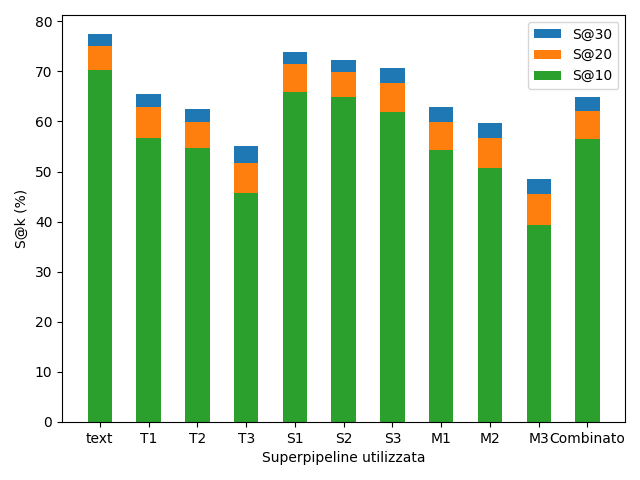
\includegraphics[width=\textwidth]{immagini/analisi/overview}
\caption{S@k misurato su ogni tipo di frase. Combinato indica S@k misurato su tutto il dataset}
\label{fig:ana_s@k}
\end{figure}


\begin{table}[H]
\centering
\begin{tabular}{cccc}
\textbf{Tipo frase} & \textbf{S@10} & \textbf{S@20} & \textbf{S@30} \\ \hline
text& 70.23& 74.98& 77.41\\
T1& 56.65& 62.87& 65.42\\
T2& 54.76& 59.98& 62.47\\
T3& 45.78& 51.75& 55.03\\
S1& 65.88& 71.46& 73.77\\
S2& 64.98& 69.9& 72.24\\
S3& 61.96& 67.59& 70.62\\
M1& 54.33& 59.82& 62.94\\
M2& 50.62& 56.63& 59.76\\
M3& 39.37& 45.52& 48.51\\
Combinato& 56.47& 62.07& 64.83\\
\end{tabular}
\caption{S@k misurato su ogni tipo di frase (risultati riportati in percentuale). Combinato indica S@k misurato su tutto il dataset}
\label{tab:ana_s@k}
\end{table}

\noindent
Da questi risultati si possono trarre alcune considerazioni:
\begin{itemize}
\item Come era facilmente prevedibile, le superpipeline più perturbate ottengono risultati visibilmente peggiori proporzionalmente al livello di perturbazione. Ciò è dato dal fatto che BERT fa uso del contesto intorno a [MASK] per provare a indovinare la parola originale. Se il contesto è sporcato, è lecito aspettarsi prestazioni più basse.

\item La generazione dei candidati risente meno dei segmentation error rispetto ai word error. Ciò potrebbe essere dovuto all'algoritmo di segmentazione WordPiece usato da BERT, che, dividendo una frase in subtoken (parti più piccole di token), potrebbe risultare particolarmente resiliente ai segmentation error. Al momento però questa è solo un'ipotesi che andrebbe approfondita e verificata.

\item Ad un maggiore valore di $k$ corrisponde naturalmente anche un incremento di $S@k$. Se da un lato questo significa che la soluzione è teoricamente presente in più casi, e quindi si ha un limite superiore più alto per le performance di correzione, dall'altro avere più candidati può portare a introdurre più errori durante la fase di scelta dei candidati. \E\ quindi necessario scegliere un valore di $k$ sufficientemente alto da produrre la soluzione, ma non così alto da far si che si confonda con gli altri candidati. Valutando la differenza fra $S@10$ e $S@20$, che è di 5,6 punti percentuali sull'intero dataset, si può concludere che l'incremento sia decisamente significativo. La differenza $S@20$ e $S@30$ corrisponde invece a 2,7 punti percentuali. Alla luce di questa osservazione, il sistema di correzione implementato utilizza un parametro $k$ pari a 20.
\end{itemize}

Quanto appena detto si può notare nel grafico della distribuzione delle soluzioni (\autoref{fig:ana_scoreorder}). Dalla distribuzione si nota come la maggior parte delle soluzioni rientri nei primi candidati, e che la presenza della soluzione al candidato n-esimo diminuisca esponenzialmente man mano che ci si allontana dalla prima posizione.


\begin{figure}[H]
\centering
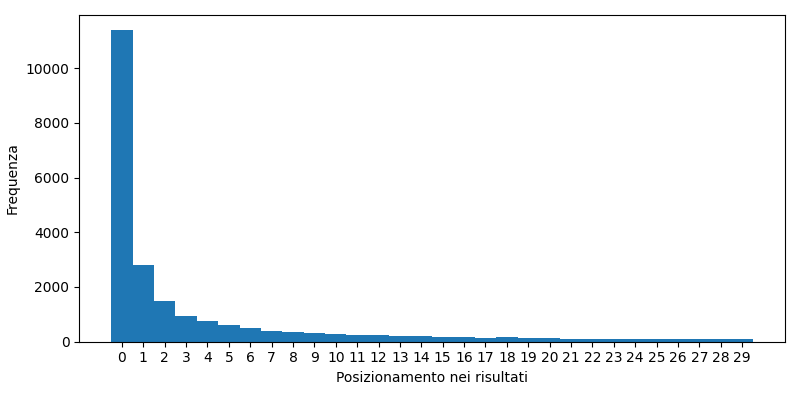
\includegraphics[width=\textwidth]{immagini/analisi/score_order_Combinato}
\caption{Distribuzione dei risultati in base all'ordinamento per probabilità prodotto da BERT di tutte le frasi del dataset (combinato). Non sono riportate le distribuzioni degli altri dataset per brevità, dato che sono pressochè sovrapponibili a quella in figura.}
\label{fig:ana_scoreorder}
\end{figure}



\section{Analisi scelta dei candidati}
\label{sec:ana_cor}

La scelta dei candidati comprende la seconda parte dello stadio candidates generation and picking e lo stadio di validation (\autoref{sec:met_tok_correct}). Data la lista dei $k$ candidati $C = [c_1,...,c_k]$ prodotti da BERT per una frase $f_{mask}$ nella quale la parola $s$ è mascherata, la scelta dei candidati deve:

\begin{enumerate}
\item Scegliere il candidato corretto se $s \in C$, ovvero se la soluzione è presente fra i candidati.

\item Non apportare alcuna correzione se $s \not\in C$, ovvero se la soluzione non è presente fra i candidati.
\end{enumerate}


\paragraph{Metriche}
Sulla base di quanto appena esposto, sono definite alcune metriche per analizzare il comportamento del sistema di correzione. Le metriche definite si dividono in due categorie:
\begin{itemize}
\item Metriche misurate nei casi in cui $s \in C$.
\item Metriche misurate nei casi in cui $s \not\in C$.
\end{itemize}
Nel caso in cui $s \in C$ sono definite le seguenti metriche:
\begin{itemize}
\item \textbf{Selezioni corrette}: percentuale dei casi in cui il sistema di correzione sceglie un candidato $c \in C$, e $c$ coincide con $s$. Ovvero, è la percentuale dei casi in cui il sistema seleziona un candidato, e il candidato selezionato è quello corretto.

\item \textbf{Selezioni errate}: percentuale dei casi in cui il sistema di correzione sceglie un candidato $c \in C$, e $c$ non coincide con $s$. Ovvero, è la percentuale dei casi in cui il sistema seleziona un candidato, e il candidato selezionato non è quello corretto.

\item \textbf{Selezioni mancate}: percentuale dei casi in cui il sistema di correzione non sceglie alcun candidato, ignorando quindi la presenza della soluzione in $C$.

\end{itemize}

\noindent
Nel caso in cui $s \not\in C$ sono definite le seguenti metriche:
\begin{itemize}
\item \textbf{Non-selezioni corrette}: percentuale dei casi in cui il sistema di correzione non sceglie alcun candidato, evitando così di introdurre un errore.

\item \textbf{Non-selezioni mancate}: percentuale dei casi in cui il sistema di correzione sceglie un candidato $c\in C$, introducendo così un errore.
\end{itemize}

\noindent
Possiamo classificare le metriche appena elencate in due categorie distinte:
\begin{itemize}
\item \textbf{Scelte Corrette:} sono tutte le scelte che il sistema prende che hanno un impatto positivo sulla correzione. Sono date dalle \textit{Selezioni corrette} e dalle \textit{Non-selezioni corrette}.

\item \textbf{Scelte Errate:} sono tutte le scelte che il sistema prende che hanno un impatto negativo sulla correzione. Sono date dalle \textit{Selezioni errate}, \textit{Selezioni mancate} e dalle \textit{Non-selezioni mancate}.
\end{itemize}

\paragraph{Risultati}
In \autoref{tab:ana_metinc} sono riportate le misurazioni per le metriche in cui la soluzione è presente fra i candidati prodotti.


Anche in questo caso, come è lecito aspettarsi, le frasi perturbate con superpipeline che introducono più rumore sono quelle che ottengono risultati peggiori, con una differenza fra i risultati migliori e peggiori contenuta entro l'8\% per quanto riguarda le selezioni corrette.
Nella discussione dei risultati si farà rifermento solo alla combinazione di tutti i tipi di frase per brevità. Tutte le considerazioni sono comunque applicabili anche per tutti gli altri tipi di frase, per i quali i risultati differiscono solo sensibilmente.\\
Come visibile nel grafico in \autoref{fig:ana_piesinc}, l'euristica di selezione del candidato produce la scelta corretta nell'85,3\% dei casi. Come mostrato in \autoref{fig:ana_levsinc}, infatti, circa l'89\% delle soluzioni si trova nella prima posizione fra i candidati ordinati per la distanza di Levenshtein. Si ricorda che l'euristica illustrata in \autoref{sec:met_errcor} sceglie sempre il candidato in prima posizione per ordinamento secondo la distanza di Levenshtein. Da questo è possibile analizzare in modo più critico i risultanti ottenuti: l'euristica identifica la soluzione nell'89\% dei casi, ma alcune soluzioni (poco più del 3\%) sono scartate dallo stadio di validazione. Il resto della percentuale di errore è dovuto all'11\% di soluzioni che si trovano dalla seconda posizione in poi nell'ordinamento per distanza di Levenshtein.


\begin{figure}[H]
\centering
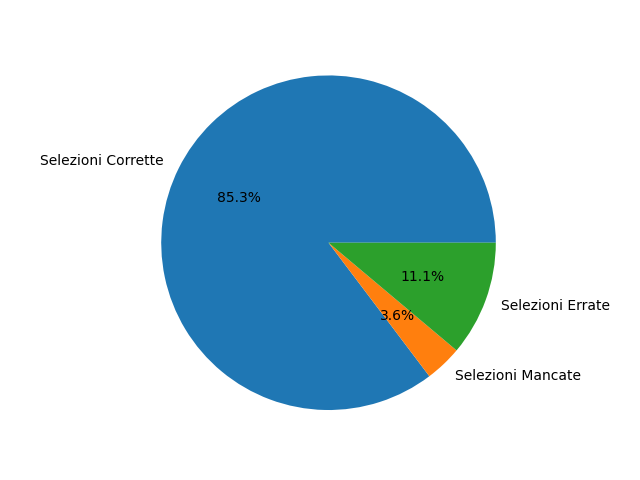
\includegraphics[width=\textwidth]{immagini/analisi/correct_combinato}
\caption{Metriche misurate per frasi in cui $s \in C$ sull'intero dataset}
\label{fig:ana_piesinc}
\end{figure}



\begin{table}[H]
\centering
\begin{tabular}{cccc}
\textbf{Pert.} & \textbf{Sel. Corrette} & \textbf{Sel. Errate} & \textbf{Sel. mancate}\\
\hline
text& 88.16& 8.8& 3.05\\
T1& 86.41& 10.0& 3.59\\
T2& 83.97& 12.02& 4.01\\
T3& 80.17& 16.69& 3.14\\
S1& 86.93& 9.15& 3.93\\
S2& 87.85& 9.31& 2.84\\
S3& 86.41& 9.53& 4.06\\
M1& 85.03& 11.2& 3.77\\
M2& 84.07& 12.05& 3.88\\
M3& 80.29& 16.12& 3.58\\
Combinato& 85.3& 11.13& 3.58\\
\end{tabular}
\caption{Metriche misurate per frasi in cui $s \in C$}
\label{tab:ana_metinc}
\end{table}




\begin{figure}[H]
\centering
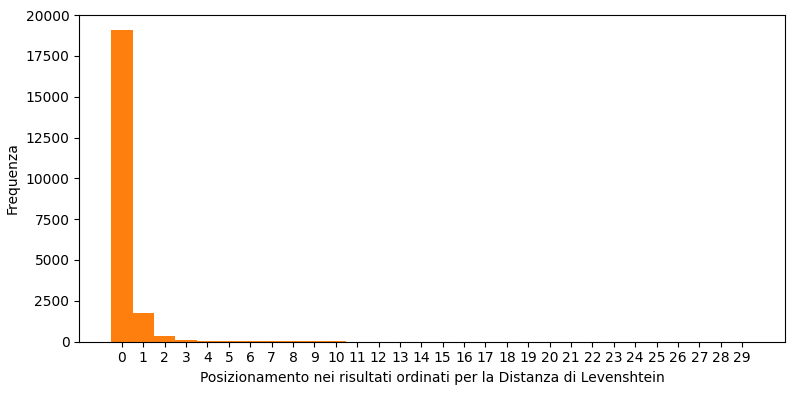
\includegraphics[width=\textwidth]{immagini/analisi/lev_pos_Combinato}
\caption{Distribuzione della posizione della soluzione all'interno dei risultati ordinati per la distanza di Levenshtein}
\label{fig:ana_levsinc}
\end{figure}

\noindent
Si analizzano ora i casi in cui la soluzione non è presente fra candidati. In \autoref{tab:ana_metninc} e in  sono riportate le statistiche per questo tipo di frasi.

\begin{table}[H]
\centering
\begin{tabular}{cccc}
\textbf{Pert.} & \textbf{N.Sel. Corrette} & \textbf{N.Sel. Mancate} &\\
\hline
text& 72.72& 27.28\\
T1& 67.71& 32.29\\
T2& 67.8& 32.2\\
T3& 64.84& 35.16\\
S1& 72.75& 27.25\\
S2& 71.96& 28.04\\
S3& 70.14& 29.86\\
M1& 68.37& 31.63\\
M2& 67.47& 32.53\\
M3& 59.65& 40.35\\
Combinato& 67.5& 32.5\\
\end{tabular}
\caption{Metriche misurate per frasi in cui $s \not\in C$}
\label{tab:ana_metninc}
\end{table}

\begin{figure}[H]
\centering
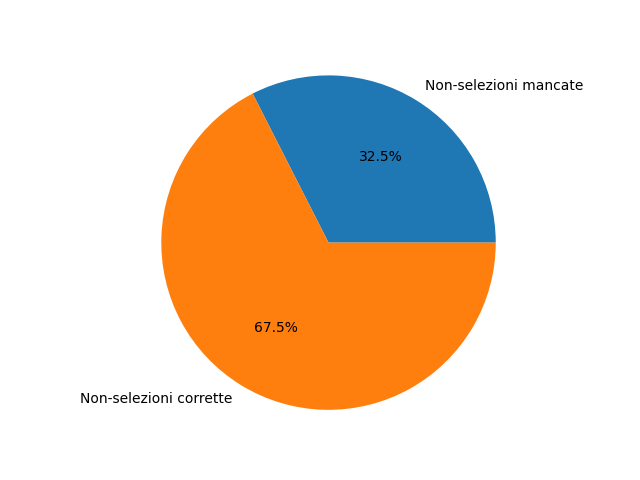
\includegraphics[width=\textwidth]{immagini/analisi/non_correct_combinato}
\caption{Metriche misurate per frasi in cui $s \not\in C$ sull'intero dataset}
\label{fig:ana_pienon}
\end{figure}

Seppur la maggior parte delle scelte che il sistema prende in questo caso sia corretta, è presente in ogni caso un'elevata percentuale di non-selezioni mancate. Si ricorda inoltre che per ogni errore viene sempre scelto un candidato per la correzione. \E\ compito dello stadio di validazione filtrare eventuali correzioni errate. La percentuale di non-selezioni errate è quindi da attribuire unicamente a questo stadio. Nell'eseguire tale analisi bisogna però anche tenere conto che nella maggioranza dei dei casi BERT riesce a produrre la soluzione fra i candidati (62,07\% dei casi, da \autoref{tab:ana_s@k}), motivo per cui è ragionevole cercare di mantenere un certo bias verso questi casi.


\begin{figure}[H]
\centering
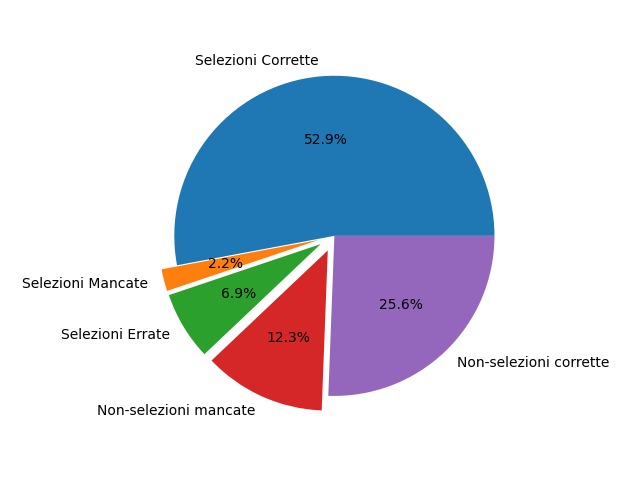
\includegraphics[width=\textwidth]{immagini/analisi/overview_scelte_combinato}
\caption{Metriche misurate sia per frasi in cui $s \not\in C$, sia per frasi in cui  $s\in C$ sull'intero dataset. Le fette esplose sono le Scelte Corrette, le rimanenti sono le Scelte Errate. }
\label{fig:ana_scelte_comb}
\end{figure}
\noindent
Per concludere questa analisi, in \autoref{fig:ana_scelte_comb} sono illustrate tutte le metriche discusse in questo capitolo. Nel comporre il grafico, si è tenuto conto della diversa cardinalità degli insiemi di frasi in cui $s\in C$ e $s\not\in C$: il peso di ogni metrica è quindi proporzionale al numero di frasi su cui è stata misurata. Si può quindi notare come il sistema di correzione effettui una scelta corretta nel 78,55\% dei casi, e prenda una scelta sbagliata nel 21,45\% dei casi (in \autoref{tab:ana_scelte_pos_neg} questa statistica è riportata per ogni tipo di frase).

\begin{table}[H]
\centering
\begin{tabular}{ccc}
\textbf{Tipo Frase} & \textbf{Scelte Corrette} & \textbf{Scelte Errate} \\ \hline
text& 84.29& 15.71\\
T1& 79.47& 20.53\\
T2& 77.5& 22.5\\
T3& 72.77& 27.23\\
S1& 82.88& 17.12\\
S2& 83.06& 16.94\\
S3& 81.14& 18.86\\
M1& 78.34& 21.66\\
M2& 76.87& 23.13\\
M3& 69.04& 30.96\\
Combinato& 78.55& 21.45\\
\end{tabular}
\caption{Percentuale di scelte positive e negative per tutti i tipi di frase}
\label{tab:ana_scelte_pos_neg}
\end{table}



